%\usepackage[top=2cm,bottom=2cm,left=1cm,right=1cm]{geometry}


\begin{titlepage}
     \begin{center}
	
\includegraphics[width=0.09\textwidth]{UNAM}\Large Universidad Nacional Autónoma de México
        	
\includegraphics[width=0.09\textwidth]{FI}\\[1cm]
        \Large Facultad de Ingeniería\\[1cm]
       % \Large División de Ciencias Básicas\\[1cm]
         \Large Laboratorio de Fundamentos de Control(6655)\\[1cm]
         %la clave antes era:4314
         \footnotesize Profesor: Salcedo Ubilla María Leonor Ing.\\[1cm]
        \footnotesize Semestre 2019-1\\[1cm]
        
       

        \Large Práctica No. 1\\[1cm]
        
           

\Large Introdcción MATLAB
        
         %Texto a la derecha
          \begin{flushright}
\footnotesize  Grupo 2\\[0.5cm]
\footnotesize Brigada: 4\\[0.5cm]
\footnotesize Rodrigo Adrián Martínez López\\[0.5cm]
\footnotesize Vivar Colina Pablo\\[0.5cm]
 \end{flushright}
    %Texto a la izquierda
          \begin{flushleft}
        \footnotesize Ciudad Universitaria Agosto de 2018.\\
          \end{flushleft}
         
          
        %\vfill
        %\today
   \end{center}
\end{titlepage}
 %agregar portada

\documentclass{article}
\usepackage[utf8]{inputenc}
\usepackage[spanish.mexico]{babel}

\title{Dispositivos}
\author{Pablo Vivar Colina}
\date{Septiembre 2017}

\usepackage{natbib}
\usepackage{graphicx}


%Circuitos
\usepackage{tikz}
\usepackage[american voltages, american currents,siunitx]{circuitikz}

%Plotting

\usepackage{pgfplots}
\pgfplotsset{width=10cm,compat=1.9} 
 %\usepgfplotslibrary{external}
\tikzexternalize 



\begin{document}


%\maketitle

%\usepackage[top=2cm,bottom=2cm,left=1cm,right=1cm]{geometry}


\begin{titlepage}
     \begin{center}
	
\includegraphics[width=0.09\textwidth]{UNAM}\Large Universidad Nacional Autónoma de México
        	
\includegraphics[width=0.09\textwidth]{FI}\\[1cm]
        \Large Facultad de Ingeniería\\[1cm]
       % \Large División de Ciencias Básicas\\[1cm]
         \Large Laboratorio de Fundamentos de Control(6655)\\[1cm]
         %la clave antes era:4314
         \footnotesize Profesor: Salcedo Ubilla María Leonor Ing.\\[1cm]
        \footnotesize Semestre 2019-1\\[1cm]
        
       

        \Large Práctica No. 1\\[1cm]
        
           

\Large Introdcción MATLAB
        
         %Texto a la derecha
          \begin{flushright}
\footnotesize  Grupo 2\\[0.5cm]
\footnotesize Brigada: 4\\[0.5cm]
\footnotesize Rodrigo Adrián Martínez López\\[0.5cm]
\footnotesize Vivar Colina Pablo\\[0.5cm]
 \end{flushright}
    %Texto a la izquierda
          \begin{flushleft}
        \footnotesize Ciudad Universitaria Agosto de 2018.\\
          \end{flushleft}
         
          
        %\vfill
        %\today
   \end{center}
\end{titlepage}
 %agregar portada

\section{Marco teórico}

\subsection{Rectificador de media onda}

El rectificador de media onda es un circuito empleado para eliminar la parte negativa o positiva de una señal de corriente alterna de lleno conducen cuando se polarizan inversamente. Además su voltaje es positivo.\citep{circuitoMediaOnda}

\begin{figure}[h!]
    \centering
    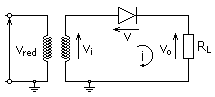
\includegraphics{Circuito_rectificador_media_onda.png}
    \caption{Caption}
    \label{fig:rectificadorMedia}
\end{figure}

\subsection{Rectificador de onda completa}

Un rectificador de onda completa es un circuito empleado para convertir una señal de corriente alterna de entrada (Vi) en corriente de salida (Vo) pulsante. A diferencia del rectificador de media onda, en este caso, la parte negativa de la señal se convierte en positiva o bien la parte positiva de la señal se convertirá en negativa, según se necesite una señal positiva o negativa de corriente continua.

Existen dos alternativas, bien empleando dos diodos o empleando cuatro (puente de Graetz).\citep{circuitoOnda}

\subsection{Tensión rectificada}

\begin{itemize}
    \item  Vo (corriente continua de salida) = Vi ( corriente alterna de entrada) = Vs/2 en el rectificador con diodos.
    \item  Vo = Vi = Vs en el rectificador con puente de Graetz.
\end{itemize}

   

Si consideramos la caída de tensión típica en los diodos en conducción, aproximadamente 0,7V; tendremos que para el caso del rectificador de doble onda la Vo = |Vi| - 1,4V.\citep{circuitoOnda}\\


\begin{figure}[h!]
    \centering
    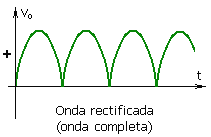
\includegraphics[scale=0.8]{OndaCompleta.png}
   % \caption{Onda Completa}
    \label{fig:my_label}
\end{figure}



\subsection{Rizado}

El rizado, algunas veces llamado fluctuación o ripple (del inglés), es el pequeño componente de alterna que queda tras rectificarse una señal a corriente continua. El rizado puede reducirse notablemente mediante un filtro de condensador, este proceso es llamado a veces "filtrar", y debe entenderse como la reducción a un valor mucho más pequeño de la componente alterna remanente tras la rectificación, pues, de no ser así, la señal resultante incluye un zumbido a 60 ó 50 Hz muy molesto, por ejemplo, en los equipos de audio.\citep{Rizado}\\

$(V_r)_{pp}$ es el voltaje de rizado de pico a pico. Recordar que $(V_r)_{pp}$ = $2\sqrt{2}(V_r)_{ef}$.\\

\begin{itemize}
    \item $I_L$es la corriente continua que demanda la carga.
    \item $f$ es la frecuencia del rizado. Esta frecuencia es igual a $f_{red}$ en un rectificador de media onda e igual a $2f_{red}$ en un rectificador de onda completa.
    \item $C$ es la capacidad del condensador.
\end{itemize}

El factor de rizado es un indicador de la efectividad del filtro y se define como:\\

\begin{equation}
     r = 100\left(\frac{V_r}{V_{cd}}\right) \quad \textrm{donde }
\end{equation}

Vr es el voltaje de rizado eficaz (rms, valor medio cuadrático)y Vcd es el valor de CD (corriente continua promedio) del voltaje de salida del filtro. Cuanto menor sea el factor de rizado, mejor será el filtro. El factor de rizado puede reducirse incrementando el valor del condensador del filtro.\citep{Rizado}\\

 \section{Material}

\begin{itemize}
    \item Resistores de distintos valores
    \item Condensadores de distintos valores
    \item 4 Diodos 1N4001
    \item Transformador de 12 [V] a 1 [A]
    
\end{itemize}

\section{Desarrollo}

\subsection{Circuito 1A}


En el desarrollo de la práctica se utilizarán 2 circuitos, uno que estará referenciado a la salida de un rectificador de onda completa que se puede apreciar en la figura \ref{fig:rectificadorPuente} y se estarán intercambiando los valores de los capacitores que se pueden observar con la etiqueta de $C_X$, y también se usó un circuito rectificador de media onda que se puede apreciar en la figura \ref{fig:rectificadorMediaOnda}, y de igual forma en los circuitos se intercambiará el valor del capacitor con la etiqueta $C_X$.\\

En el gráfico \ref{fig:circuito1A} se pueden apreciar las señales AC y DC que se ingresaron en el rectificador de onda completa cuando el capacitor $C_X$ es de $0.04 [\mu F]$, se puede ver el desplazamiento de 10 [V].

\begin{figure}[ht!]
    \centering
    \begin{circuitikz}
    
        \draw (0,0) node [transformer](T){}
        
       (2,0)to[D,v=]   (3,-1.1)
       (1,-1.1)to[D,v=]  (2,0) 
         (1,-1.1)  to[D,v=](2,-2.1)
          (2,-2.1) to[D,v=] (3,-1.1)
         %(0,0) node {"+"}
          
          %Para el puente
          (1,0)--(2,0)
          (1,-2.1)--(2,-2.1)
          
          %para rectificador
          (3,-1.1)--(4,-1.1)
          (1,-1.1)--(1,-3.1)
          (1,-3.1)--(4,-3.1)
          
         
         %notas de rectificador
          (3.5,-0.9) node {+}
           (3.5,-2.8) node {-}
           
           
            (4,-1.1)--(6,-1.1)
           (4,-3.1)--(6,-3.1)
           
           % (4,-0.5) node {$0.04 [\mu F]$}
           (4,-1.1)to[C,l=$C_1$](4,-3.1)
           (5.5,-0.5) node {$[1k \Omega]$}
             %(5.5,-1.1)to[R,l=$R_{10}$](5.5,-3.1)
          
        ;
        
        
    \end{circuitikz}
    \caption{Rectificador tipo Onda Completa tipo Puente}
    \label{fig:rectificadorPuente}
\end{figure}

\begin{figure}
    \centering
    
   
\begin{tikzpicture}
\begin{axis}[
    axis lines = left,
    xlabel = $t$,
    ylabel = {$V_{pp}$},
]

%señal DC
\addplot [
    domain=(0*3.14159):+(1*3.14159), 
    samples=100, 
    color=blue,
]
{15*sin(deg(x))};
\addlegendentry{$15 V_{pp} DC$}

\addplot [
    domain=(1*3.14159):+(2*3.14159), 
    samples=100, 
    color=blue,
]
{-15*sin(deg(x))};
%\addlegendentry{$15 V_{pp}$}

\addplot [
    domain=(2*3.14159):+(3*3.14159), 
    samples=100, 
    color=blue,
]
{15*sin(deg(x))};
%\addlegendentry{$15 V_{pp}$}

%señal AC
\addplot [
    domain=(0*3.14159):+(1*3.14159), 
    samples=100, 
    color=red,
]
{15*sin(deg(x))-10};

 \addplot [
    domain=(1*3.14159):+(2*3.14159), 
    samples=100, 
    color=red,
]
{-15*sin(deg(x))-10};
%\addlegendentry{$15 V_{pp}$}

\addplot [
    domain=(2*3.14159):+(3*3.14159), 
    samples=100, 
    color=red,
]
{15*sin(deg(x))-10};
%\addlegendentry{$15 V_{pp}$}
 %Fin plots
 
    color=blue,
 
\end{axis}
\end{tikzpicture}

 \caption{Señales en circuito 1A}
    \label{fig:circuito1A}
\end{figure}



%\subsection{Circuito 2A}

\begin{figure}[ht!]
    \centering
    \begin{circuitikz}
    
        \draw (0,0) node [transformer](T){};
        \draw  (1,0) to[D,v=D](3,0);  
        \draw (3,0)to[C,l=$C_X$](3,-2.1)
        (1,-2.1)--(3,-2.1);
        \draw  (5,0) to[R,l=$R_{10}$](5,-2.1)
        (3,0)--(6,0)
        (3,-2.1)--(6,-2.1)
        
        (3,0.5) node {$0.04 [\mu F]$}
        (5,0.5) node {$1 [k \Omega]$}
        ;
        
    \end{circuitikz}
    \caption{Rectificador media Onda}
    \label{fig:rectificadorMediaOnda}
\end{figure}

\subsection{Circuito 2A}


En la figura \ref{fig:circuito2A} se puede apreciar el comportamiento del circuito rectificador de media onda cuándo el capacitor $C_X$ tiene un valor de $0.04 [\mu F]$ en el circuito \ref{fig:rectificadorMediaOnda}

\begin{figure}
    \centering
    
   
\begin{tikzpicture}
\begin{axis}[
    axis lines = left,
    xlabel = $t$,
    ylabel = {$V_{pp}$},
]

%señal DC
\addplot [
    domain=(0*3.14159):+(1*3.14159), 
    samples=100, 
    color=blue,
]
{15*sin(deg(x))};



\addplot [
    domain=(1*3.14159):+(2*3.14159), 
    samples=100, 
    color=blue,
]
{0};


\addplot [
    domain=(2*3.14159):+(3*3.14159), 
    samples=100, 
    color=blue,
]
{15*sin(deg(x))};
\addlegendentry{$15 V_{pp} DC$}

%Señal AC
\addplot [
    domain=(0*3.14159):+(1*3.14159), 
    samples=100, 
    color=red,
]
{15*sin(deg(x))-6};



\addplot [
    domain=(1*3.14159):+(2*3.14159), 
    samples=100, 
    color=red,
]
{0-6};


\addplot [
    domain=(2*3.14159):+(3*3.14159), 
    samples=100, 
    color=red,
]
{15*sin(deg(x))-6};




 
\end{axis}
\end{tikzpicture}

 \caption{Señales en circuito 2A}
    \label{fig:circuito2A}
\end{figure}



%\subsection{Circuito 1B}

%Para éste circuito se utilizó un capacitor de $10 \mu F$ en la figura \ref{fig:rectificadorPuente} y se apreciaron las señales expuestas en la figura \ref{fig:circuito1B}


%\begin{figure}
 %   \centering
    
   
%\begin{tikzpicture}
%\begin{axis}[
 %   axis lines = left,
  %  xlabel = $t$,
  %  ylabel = {$V_{pp}$},
%]

%señal DC
%\addplot [
 %   domain=(0.23*3.14159):+(0.7*3.14159), 
  %  samples=100, 
   % color=blue,
%]
%{15*sin(deg(x))};

%\addplot [
 %   domain=(2*0.23*3.14159):+(2*0.7*3.14159), 
 %   samples=100, 
 %   color=blue,
%]
%{15*sin(deg(x))};



%Señal AC
%\addplot [
 %   domain=(0*3.14159):+(1*3.14159), 
  %  samples=100, 
   % color=red,
%]
%{15*sin(deg(x))-6};



%\addplot [
%    domain=(1*3.14159):+(2*3.14159), 
%    samples=100, 
%    color=red,
%]
%{0-6};


%\addplot [
 %   domain=(2*3.14159):+(3*3.14159), 
  %  samples=100, 
   % color=red,
%]
%{15*sin(deg(x))-6};




 
%\end{axis}
%\end{tikzpicture}

 %\caption{Señales en circuito 1B}
 %   \label{fig:circuito1B}
%\end{figure}

%\subsection{Circuito 2B}

%\subsection{Circuito 1C}

%\subsection{Circuito 2C}

%\subsection{Circuito 2D}

%\subsection{Circuito 2D}

%\subsection{Circuito 1E}

%\subsection{Circuito 2E}

%\subsection{Circuito 1F}

%\subsection{Circuito 2F}



%######## AQUI VA LA PRACTICA ########

%mbi armiya naroda! :D
%https://www.youtube.com/watch?v=3D5-pleHkdk

\section{Conclusiones}

En la práctica se observó la capactidad de los capacitores y resitores de alterar el rizo de la señal, esto es de importancia ya que con la correcta elección de éstos componentes se puede filtrar la salida de un transformador para crear un voltaje continuo pulsante, se hizo un experimento extra en dónde se colocó un potenciómetro en el circuito rectificador de onda completa  y se eligió un valor para hacer que el rizo fuera lo mínimo posible el valor de resitencia fue de 40 y 90 $[\Omega]$ para un capacitor de 1000 $[\mu F]$.



\bibliographystyle{plain}
\bibliography{referencias8.bib}

\end{document}